\documentclass[11pt,a4paper]{article}

\usepackage{titling}
\usepackage[hidelinks]{hyperref}
\usepackage{graphicx}
\usepackage{grffile}
\usepackage{float}
\usepackage{geometry}
\usepackage{listings}

\newcommand{\subtitle}[1]{
  \posttitle{
    \par\end{center}
    \begin{center}\large#1\end{center}
    \vskip0.5em}
}

\begin{document}


\title{Hyper Perform\\ Testing Document}
\subtitle{ Repository: \url{https://github.com/claudioMDS/hyper-perform}}
\begin{figure}
			\centering
			
\includegraphics[height=200px]{../Images/CodusMaximus_logo.jpg}
\end{figure}

	
\author{
	\textbf{Developers:} \\
	Claudio Da Silva	\emph{14205892}	\\
	Rohan Chhipa		\emph{14188377}	\\
	Avinash Singh		\emph{14043778}	\\
	Jason Gordon		\emph{14405025}	\\\\
}

\date{\textbf{Updated \today}}

\maketitle
\thispagestyle{empty}
\pagebreak

\tableofcontents
\pagebreak

\section{Introduction}

This document explains implementation of unit tests which were used to test each component in an isolated environment. It also includes an overview of the technologies used as well as instructions on how to execute these tests. \\ 

\section{Technologies}

Since the system was primarily coded with Java we used JUnit to carry out the unit tests for each of the components. We also used Spring to allow us to use dependency injection within each test, this allows us to easily inject mocks and test components in an isolated environment. \\

Another technology which proved useful was a Mock Dispatcher framework which ships with RESTEasy. The mock dispatcher allows one to easily and efficiently test REST API's without having to deploy the component to an application server.

\section{Execution of unit tests}
The project was developed using Maven as a build tool. Thus each unit test can be easily found within the $src/test$ directory of the project. To run the unit tests simply run the following command on terminal: \\

$mvn\ clean\ test$ \\

All the necessary dependencies for the project will be automatically downloaded. \textbf{Note:} This process of downloading all the project dependencies might consume large amounts of data.

\section{Test items}
At this point in the project the following features will be tested:
\begin{itemize}
	\item The GitListener which receives events from GitHub.
	\item GitPushEvent which is a POJO that contains information regarding a GitHub event.
	\item CalendarListener which receives events from Google Calender service.
	\item The error codes and exceptions raised when accessing an invalid REST URL.
\end{itemize}

Each of these components have dependencies on features such as the messaging queue. All of these features are mocked out to ensure each component is tested in isolation. These features were mocked through dependency injection which was provided by Spring. \\

\section{Features that will not be tested}

Features that have been provided by frameworks will not be tested. Operations such as adding an object to a messaging queue will not be tested.

\section{Components to be mocked}
\begin{itemize}
	\item The JPA entity manager was the first component that was mocked. When testing the persistibility of the POJO's it would be best if the transactions do not affect the database. Thus every transaction that occurs with the mocked entity manager will leave the database system intact and unaffected. An alternate approach could have been to use an in-memory database such as the one provided by H2 however this was not deemed necessary. \\
	
	\item The second component to be mocked was the messaging queue provided by ActiveMQ. Once again we do not wish to have unnecessary objects in our queue that might affect actual program execution thus the default queue is replaced with a queue that does not retain objects. \\
	
	\item When testing the event listeners we can't wait for the event emitting systems to send out an event. So we send mock events to the listeners while testing, these mock events are structured in the same manner as there real-world counterparts.
\end{itemize}

\section{Sample tests}
The following figure is one of the GitListener Event tests.

\begin{figure}[H]
	\begin{center}
		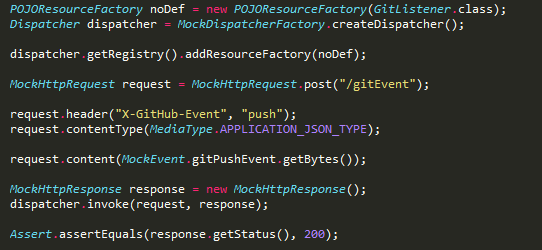
\includegraphics[scale=1.0]{../Images/sample1.png}
		\caption{GitListener Push event test}
	\end{center}
\end{figure}

In the above figure the $POJOResourceFactory$ and $Dispatcher$ are used to start up an embedded server which will allow for calls to be made to a particular URL, in this case $\backslash$ gitEvent. \\

A post request is created and has the mock event as its content. This post request mirrors the post requests made by GitHub when sending events. Once the mock event data is loaded into the request the request is sent. At the end the response objects HTTP status code is checked. This is checked in an assert statement, the value of the response should be 200 to indicate a successful retrieval. \\

\begin{figure}[H]
	\begin{center}
		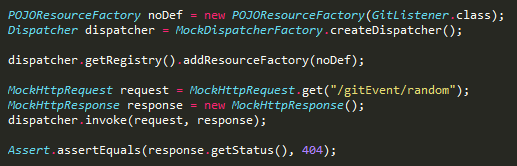
\includegraphics[scale=1.0]{../Images/sample2.png}
		\caption{Exception handler for invalid URLs}
	\end{center}
\end{figure}

\end{document}